% --- IMPORTANT -------------------------------------
%
% Make a folder 'theme' linking to the folder
%  /nfs/users2/liney/LaTeX/LU
% by the command
%  ln -s /nfs/users2/liney/LaTeX/LU/ theme
%
% Note that the footer height is excessive since
% some poster printers (e.g. the one at LU Fysicum)
% don't print to the end of the poster (cut off).
%
% ---------------------------------------------------

\documentclass[final,hyperref={pdfpagelabels=true},notheorems]{beamer}
\usepackage{xltxtra}
% Choose an otf-font - xelatex only!!!
\setmainfont{Frutiger LT Std}

\usepackage{grffile}
\mode<presentation>{\usepackage{theme/beamerthemelund}}
\usepackage[english]{babel}
% Choose the corresponding input encoding of your tex-file - only if you use pdflatex instead of xelatex!
% \usepackage[latin1]{inputenc}
% \usepackage[utf8]{inputenc}
%
\usepackage{amsmath,amsthm, amssymb,latexsym,pifont}
% \usepackage[tight,FIGTOPCAP]{subfigure}
\usepackage[tight]{subfigure}
\usefonttheme[onlymath]{serif}
\boldmath
\usepackage[orientation=portrait,size=a0,scale=1.6,debug]{beamerposter}
% change list indention level
% \setdefaultleftmargin{3em}{}{}{}{}{}

\usepackage{natbib}
\bibstyle{nature}
\newcommand{\newblock}{}

%\usepackage{snapshot} % will write a .dep file with all dependencies, allows for easy bundling

% \usepackage[labelfont=bf,labelsep=period]{caption}

% \usepackage{array,booktabs,tabularx}
% \newcolumntype{Z}{>{\centering\arraybackslash}X} % centered tabularx columns
% \newcommand{\pphantom}{\textcolor{lundlightgray}} % phantom introduces a vertical space in p formatted table columns

\listfiles

%%%%%%%%%%%%%%%%%%%%%%%%%%%%%%%%%%%%%%%%%%%%%%%%%%%%%%%%%%%%%%%%%%%%%%%%%%%%%%%%%%%%%%
% \graphicspath{{figures/}}
 
\title{\huge Some Really Catching Title}
\author{\vskip0.5ex\textbf{Main Author}, Co-Author 1, Co-Author 2, etc.}
\institute[Lund University]{\textit{Nanometer Structure Consortium, Lund University, Box 118, SE-221 00 Lund, Sweden}%\\ \textit{}
}
\date[25 July 2010]{25 July 2010}

\renewcommand{\authorFig}{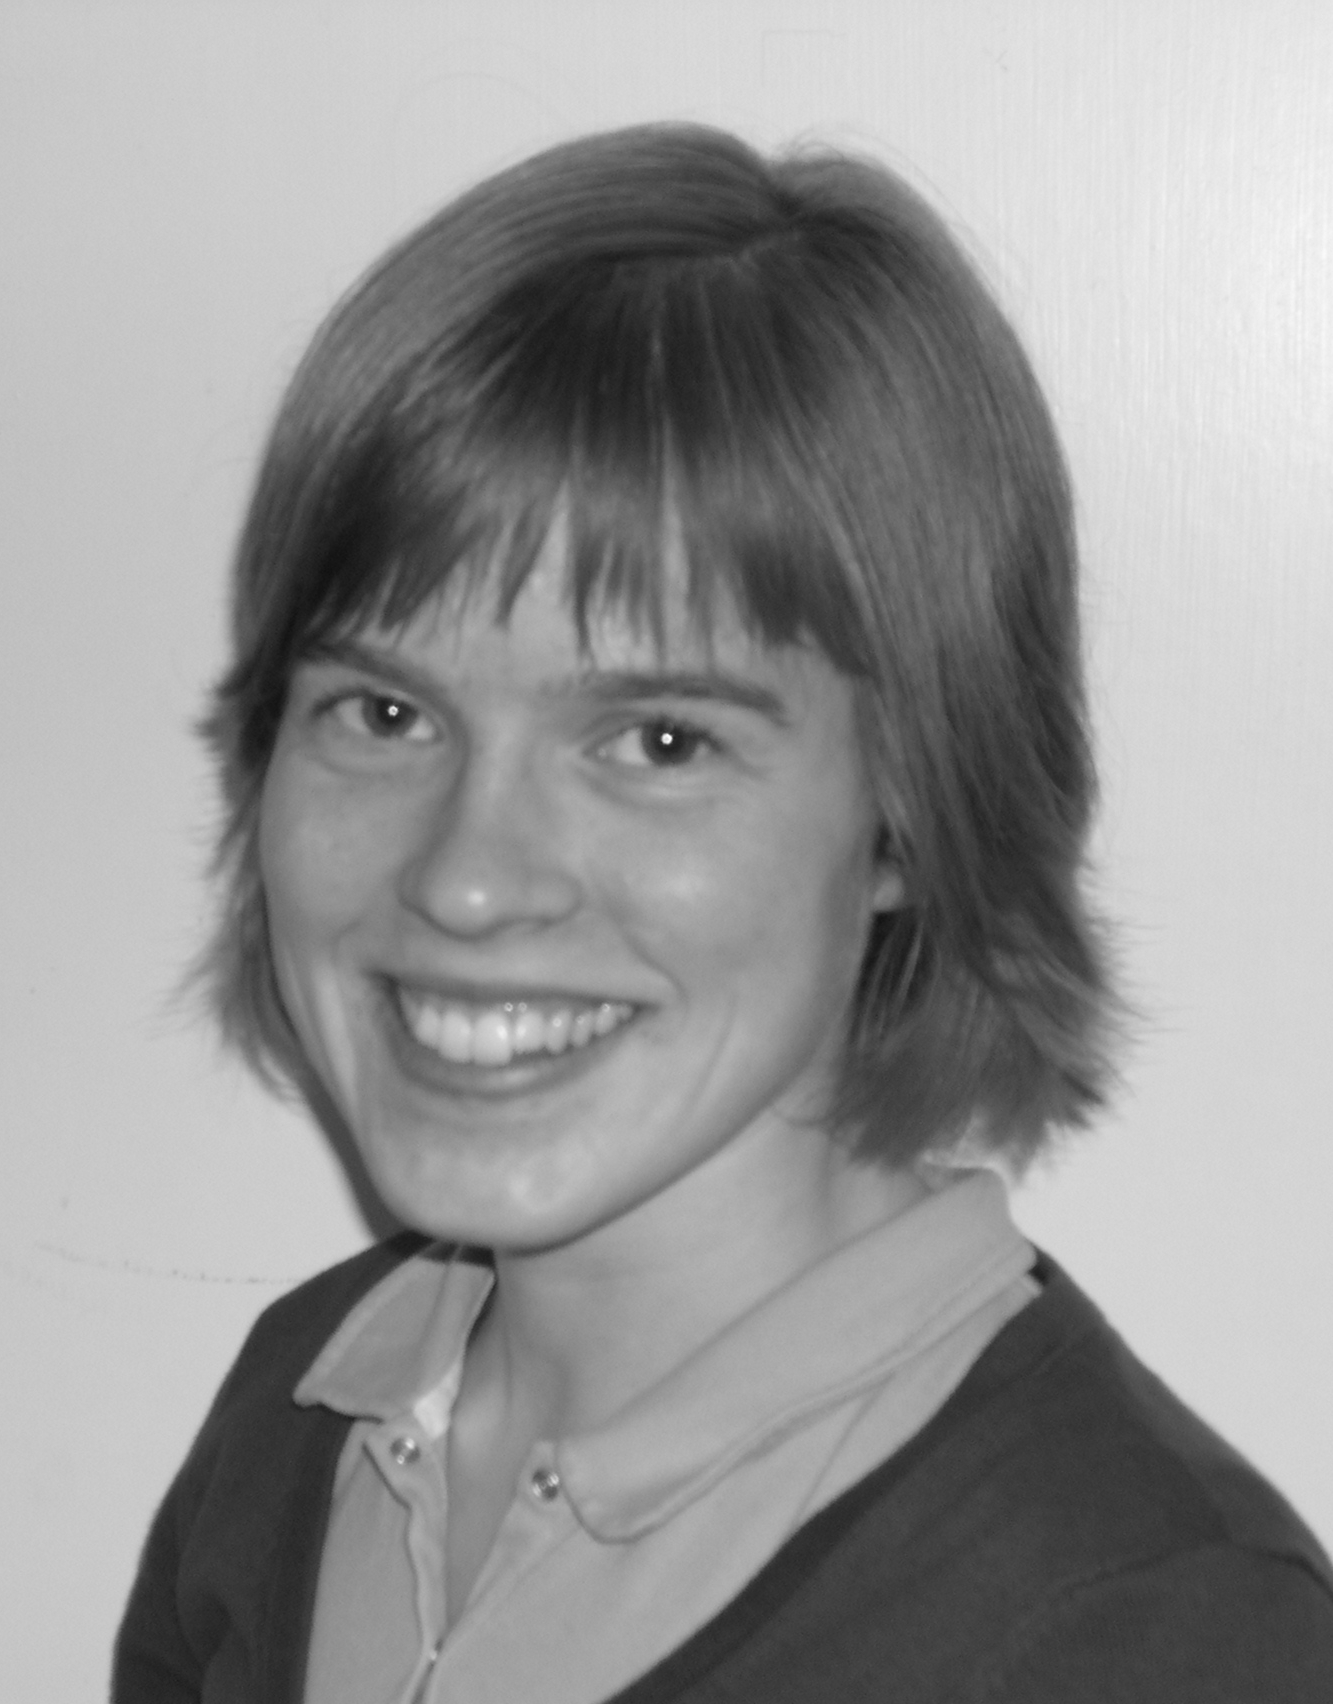
\includegraphics[width=\linewidth]{theme/figs/LHK_BW.jpg}}
\renewcommand{\universityLogo}{
\includegraphics[width=.8\linewidth]{theme/figs/LundUniversity_C2line_CMYK.png}}
\renewcommand{\footerLeft}{\textsf{Opportunity/place of poster presentation}}
\renewcommand{\footerRight}{\texttt{liney@matfys.lth.se}}

%%%%%%%%%%%%%%%%%%%%%%%%%%%%%%%%%%%%%%%%%%%%%%%%%%%%%%%%%%%%%%%%%%%%%%%%%%%%%%%%%%%%%%
\newlength{\columnheight}
\setlength{\columnheight}{99cm}


%%%%%%%%%%%%%%%%%%%%%%%%%%%%%%%%%%%%%%%%%%%%%%%%%%%%%%%%%%%%%%%%%%%%%%%%%%%%%%%%%%%%%%
\begin{document}
\begin{frame}
%   \vskip1cm
  \begin{columns}
    % ---------------------------------------------------------%
    % Set up a column 
    \begin{column}{.32\textwidth}
      \begin{beamercolorbox}[center,wd=\textwidth]{postercolumn}
        \begin{minipage}[T]{.95\textwidth}  % tweaks the width, makes a new \textwidth
          \parbox[t][\columnheight]{\textwidth}{ % must be some better way to set the the height, width and textwidth simultaneously
            % Since all columns are the same length, it is all nice and tidy.  You have to get the height empirically
            % ---------------------------------------------------------%
            % fill each column with content
            \begin{alertblock}{Motivation\phantom{Gg}}
              Experimental results of electron transport through InSb nanowires~\cite{NilssonNL2009} indicated signatures of Wigner crystallization. Theoretical modelling needed to support or reject the hypothesis.
            \end{alertblock}
            \vfill
            \begin{block}{Wigner Crystallization\phantom{Gg}}
              \begin{itemize}
               \item Wigner crystallization is the localisation of electrons, when interaction energy dominates kinetic energy.% -- it is a many-body phenomenon.
               \item Predicted by Wigner in 1934~\cite{wigner1934}.
               \item Not yet observed in semiconductor nanowires.
               \item We report signatures of Wigner crystallization and the possibility of detecting full Wigner crystallization in semiconductor nanowires.
              \end{itemize}
            \end{block}
            \vfill
            \begin{block}{Experiments and Modelling\phantom{Gg}}
              \begin{figure}
                \subfigure[InSb wire on a SiO$_\text{2}$ capped highly doped Si substrate, with gold contacts (source, drain) grown across. The length of the quantum dot is $l=$~160~nm.]{
%                   \includegraphics[width=0.9\textwidth]{figs/SEMimage.png}
                }
                \\[1em]
                \subfigure[Modelling of the wire.]{
%                   \includegraphics[width=0.9\textwidth]{figs/schemFigWire.pdf}
                }
                \caption{(a) SEM image of a 160~nm long, 70~nm diameter InSb nanowire quantum dot device, and (b) a schematic diagram of the modelling of a nanowire of length $l$ and dielectric constant $\epsilon_\text{in}$.}
                \label{fig:wire}
              \end{figure}
              \begin{itemize}
                \item Measurements of electron transport~\cite{NilssonNL2009}:
                \begin{itemize}
                  \item InSb nanowires (see Fig.~\ref{fig:wire}(a));
                  \item Diameter 70~nm and lengths 70~nm and 160~nm;
                  \item At temperature 300~mK.
                \end{itemize}
                \item Model electron transport through the wire:
                \begin{itemize}
                  \item \textbf{1D model.} We derive the effective 1D Coulomb interaction by modelling the wire as an infinite cylinder of 70~nm diameter and relative permittivity $\epsilon_\text{in}=\epsilon_\text{InSb}=$~16, embedded in a medium of relative permittivity $\epsilon_\text{out}$, and integrating out the radial and angular degrees of freedom. The $\epsilon_\text{out}$ is used as a fitting parameter to experiments. It is taken as a weighted average of the substrate and the surrounding air, with the screening of the gold contacts taken into account;
                  \item Electron states in the wire calculated by the \textbf{configuration interaction method} (many-body calculation);
                  \item Combined with \textbf{master equation approach} (transport simulation). %properties)
                \end{itemize}
              \end{itemize}
            \end{block}
          }
        \end{minipage}
      \end{beamercolorbox}
    \end{column}
    % ---------------------------------------------------------%
    % end the column


    % ---------------------------------------------------------%
    % Set up a column 
    \begin{column}{.32\textwidth}
      \begin{beamercolorbox}[center,wd=\textwidth]{postercolumn}
        \begin{minipage}[T]{.95\textwidth} % tweaks the width, makes a new \textwidth
          \parbox[t][\columnheight]{\textwidth}{ % must be some better way to set the the height, width and textwidth simultaneously
            % Since all columns are the same length, it is all nice and tidy.  You have to get the height empirically
            % ---------------------------------------------------------%
            % fill each column with content
            \begin{block}{Results\phantom{Gg}} %\vspace*{0.3ex}
              \begin{itemize}
                \item Experiments and simulations:
                \begin{itemize}
                  \item Fit the width of the Coulomb diamonds via $\epsilon_\text{out}$ (dielectric constant of medium outside wire);
                  \item Other features of the charge stability diagrams which are not fitted by hand, match very well between theory and experiment, both for 70~nm (not shown) and 160~nm (compare Figs.~\ref{fig:cond}(b) and (c), e.g. the lines marked by \ding{193} and \ding{195}).
                \end{itemize} \vskip1.4ex
                \item No Wigner crystallization: %\newline
                \begin{columns}
                  \begin{column}{0.3\linewidth} \centering\vspace*{0.2ex}
%                     \hspace*{1em}\includegraphics[height=12cm]{figs/densplot_L070.pdf}
                    \vskip1ex
                  \end{column}
                  \begin{column}{0.65\linewidth}
                    \begin{itemize}
                      \item Interaction is non-essential;
                      \item Independent particle approximation: Many-particle energy levels in the wire can be found by simply ordering the electrons into single-particle levels, applying the Pauli principle;
                    \end{itemize}
                  \end{column}
                \end{columns}
                \begin{itemize}
                  \item The energy needed to excite a single electron from the ground state to the 1st excited single-electron state, $\Delta E_1$, is approximately the same as the energy difference between the 2-electron ground and 1st excited state, $\Delta E_2$ (see inset in Fig.~\ref{fig:cond}(a));
                  \item \textsl{Experimental recognition:} Distance between lines \ding{192} and \ding{193} is the same as between lines \ding{194} and \ding{195}.
                \end{itemize} \vskip1.4ex
                \item Onset of Wigner crystallization: %\newline
                \begin{center} \vspace*{0.2ex}
%                   \includegraphics[height=12cm]{figs/densplot_L160.pdf}
                \end{center}
                \begin{itemize}
                  \item Interaction is non-negligible, simple single-electron calculations will not do;
                  \item $\Delta E_1\gg\Delta E_2$ (see inset in Fig.~\ref{fig:cond}(b)).
                  \item \textsl{Experimental recognition:} Distance between lines \ding{192} and \ding{193} is considerably larger than the distance between lines \ding{194} and \ding{195}.
                \end{itemize} \vskip1.4ex
                \item Wigner crystallization: %\newline
                \begin{center} \vspace*{-2.3ex}
%                   \includegraphics[height=12cm]{figs/densplot_L300.pdf}
                \end{center}
                \begin{itemize}
                  \item Simulations only, no successful experiments yet!
                  \item The lowest singlet and triplet states are practically the same, as a result of the localisation -- the relative spin orientation of the two electrons does not matter as they are separated;
                  \item \textsl{Experimental recognition (in theory):} Lines \ding{194} and \ding{195} cannot be distinguished as two different lines (see Fig.~\ref{fig:cond}(d)), i.e. the distance between lines \ding{192} and \ding{193} is smaller than the distance from line \ding{194} to the next discernible line that leads all the way to the $N=2$ Coulomb diamond.
                \end{itemize}
              \end{itemize}
            \end{block}
          }
        \end{minipage}
      \end{beamercolorbox}
    \end{column}
    % ---------------------------------------------------------%
    % end the column


    % ---------------------------------------------------------%
    % Set up a column 
    \begin{column}{.32\textwidth}
      \begin{beamercolorbox}[center,wd=\textwidth]{postercolumn}
        \begin{minipage}[T]{.95\textwidth} % tweaks the width, makes a new \textwidth
          \parbox[t][\columnheight]{\textwidth}{ % must be some better way to set the the height, width and textwidth simultaneously
            % Since all columns are the same length, it is all nice and tidy.  You have to get the height empirically
            % ---------------------------------------------------------%
            % fill each column with content
            \begin{block}{Results (cont.)\phantom{Gg}}
              \begin{figure}
%                 \includegraphics[width=0.9\textwidth]{figs/cond_L070L160L300.png}
                \caption{Charge stability diagrams: Differential conductance ($\mathrm dI/\mathrm dV_\text{sd}$) vs. source-drain bias voltage ($V_\text{sd}$) and gate energy ($E_g$) or gate voltage ($V_{bg}$). \linebreak
                (a) Simulations of a $l=$~70~nm wire. (b) Simulations of a $l=$~160~nm wire. (c) Experimental results for a  $l=$~160~nm wire. (d) Simulations of a $l=$~300~nm wire. In all panels, lines corresponding to transport through the 1- and 2-electron ground state and 1st excited state are labelled by the symbols \ding{192}, \ding{193}, \ding{194} and \ding{195} (see legend). The separation of these lines provides the excitation energies from the 1- and 2-electron ground state. In panels (a) and (b) these are marked by $\Delta E_1$ and $\Delta E_2$, respectively.}
                \label{fig:cond}
              \end{figure}
            \end{block}
            \vfill
            \begin{exampleblock}{Summary\phantom{Gg}}
              We have modelled electron transport through InSb nanowires. Our theoretical results are consistent with the existing experimental data. They confirm the detection of the onset of Wigner crystallization, and predict at which wire length complete Wigner crystallization is to be expected.
            \end{exampleblock}
            \vfill
            \begin{block}{References\phantom{Gg}}
              \small
%               \bibliographystyle{nature}
%               \bibliography{refs}
              \begin{thebibliography}{1}
              \bibitem{NilssonNL2009}
              Nilsson, H.~A., Caroff, P., Thelander, C., Larsson, M., Wagner, J.~B.,
                Wernersson, L.-E., Samuelson, L., and Xu, H.~Q.
%               \newline
              {\em Nano Lett.}{ \textbf{9}}({9}), 3151 ({2009}).
              \bibitem{wigner1934}
              Wigner, E.
              {\em Phys. Rev.}{ \textbf{46}}, 1002 (1934).
              \end{thebibliography}
            \end{block}
          }
          % ---------------------------------------------------------%
          % end the column
        \end{minipage}
      \end{beamercolorbox}
    \end{column}
    % ---------------------------------------------------------%
    % end the column
  \end{columns}
  \vskip0.5ex
  %\tiny\hfill\textcolor{ta2gray}{Created with \LaTeX \texttt{beamerposter}  \url{http://www-i6.informatik.rwth-aachen.de/~dreuw/latexbeamerposter.php}}
  \tiny\hfill{Created with \LaTeX{} \texttt{beamerposter}  \hskip1em}
\end{frame}
\end{document}


%%%%%%%%%%%%%%%%%%%%%%%%%%%%%%%%%%%%%%%%%%%%%%%%%%%%%%%%%%%%%%%%%%%%%%%%%%%%%%%%%%%%%%%%%%%%%%%%%%%%
%%% Local Variables: 
%%% mode: latex
%%% TeX-PDF-mode: t
%%% End:
